\chapter{An Integral Review for Integration}
Eventually, integrals will become a core aspect of this coursework.
Therefore, to prepare students for upcoming mathematical prerequisite knowledge, we aim to review some core aspects of integrals here.
If you have never learned integrals before, you probably should not be here; and, if you would still like to digest the contents here, you may want to consult other resources along with this one, as this resource will only discuss a summary of integral techniques.

\section{A Brief Review of An Integral}
The most explicit interpretation of an integral is the area under curve: provided some curve that represents a single-variate function $f$, the area under its curve from $x = a$ to $x = b$ is an integral: $\int_a^b f(x) \,dx$.

Let us discuss this interpretation furthermore by discussing some methodologies within our scope for approximating the area under curve.
\begin{center}
    \begin{figure}
        \centering
        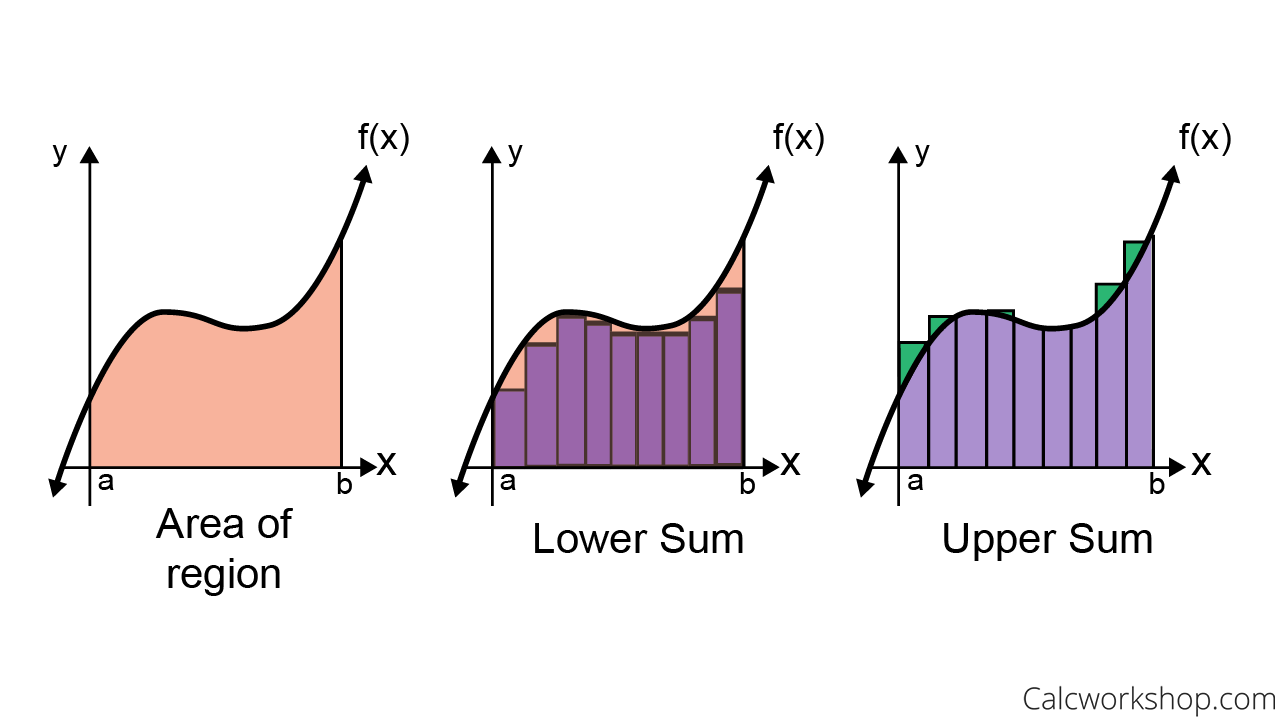
\includegraphics[width=0.7\textwidth]{figs/ln10/riemann-sums-area-distances.png}
    \end{figure}
\end{center}

In the above figure, the ``Lower Sum'' and ``Upper Sum'' techniques (formally known as Reimann Sums) attempt to approximate the area under curve with the following algorithm:
\begin{enumerate}
    \item Decide the width of the rectangles that will fill the area under curve (or, overfill).
    \item Decide the height of the rectangle based on either the curve height at the left or right end of the rectangle. Alternatively, we may also choose either the lower one or the higher one (respectively leading to the ``Lower Sum'' and ``Higher Sum'' techniques above).
    \item Sum the areas of these rectangles.
\end{enumerate}
We consider this as a discrete operation. Discrete here means that the mathematical operations is done on a non-continuous number line that does not contain every possible number. For example, by deciding the width of rectangle, we also decide to skip looking at the function values of any number that is not the rectangle width.
However, as you may have noted, discrete operations do not provide a great approximation and may take a lot of computation as the number of rectangles increase.

What if there is, instead, a continuous method of doing so, such that we can consider rectangles of infinitesimal widths and sum up their areas?
Such is the operation that we call integrals.
In other words, integral operations are the discrete summation techniques we see in the above picture, except we now use infinitesimal-width rectangles such that we can most accurately portray the area under curve with the sum of those rectangles.
This shows us that integrals are actually the analogy of summations in a continuous space.

While the summation methods using $n$ rectangles to approximate the area under curve within $[a, b]$ may be simplified as a summation:
\[
    \sum_{i=0}^{n - 1} \frac{b - a}{n} f(a + i \times \frac{b - a}{n})
\]
The integral version of such method is instead written as:
\[
    \int_a^b f(x) \,dx = \lim_{n\to\infty} \sum_{i=0}^{n - 1} \frac{b - a}{n} f(a + i \times \frac{b - a}{n})
\]
We will introduce its mathematical operations in the coming section.

\section{Computing An Integral}
To compute an integral $\int_a^b f(x) \,dx$, we first find the antiderivate of function $f$ (which we would call $F$), then we would compute the value of integral as $F(b) - F(a)$. \\
The above very, very rough summary forgets to address several subtleties:
\begin{enumerate}
    \item The definition of antiderivative and the computations required to find it.
    \item The reason why we may claim the value of $\int_a^b f(x) \,dx$ to be the difference $F(b) - F(a)$.
    \item What do we do when there exists a point $x' \in [a, b]$ at which the function $f$ is not defined at.
\end{enumerate}

Let us address the above concerns one by one to validify the summarizing statement.

First of all, the antiderivaitve $F$ of a function $f$ is a function such that $\dv{F}{x} = f(x)$.
Provided so, the antiderivative of any function $f$ is not unique. Let us proceed with a proof, or, an argument to prove or disprove a mathematical statement:
\begin{ln-explain}{Antiderivative of Function $f(x)$ is Non-Unique}{}
    Suppose that the function $f$ already has an antiderivative $F(x)$.
    Then, let $C$ be a scalar, real constant. We may see that:
    \begin{align*}
        \dv*{}{x} (F(x) + C) &= f(x) + \dv*{}{x} C \\
        &= f(x) + 0 = f(x)
    \end{align*}
\end{ln-explain}
Usually, then, we denote the antiderivative of $f(x)$ as $F(x) + C$ for the above reason.

Meanwhile, the computation of integral from antiderivatives is secured by a famous theorem that we introduce below:
\begin{ln-theorem}{Fundamental Theorems of Calculus}{}
    \textit{\textbf{The first fundamental theorem of calculus.}}
    Let $f$ be a continuous real-valued function defined on a closed interval $[a, b]$. Let $F$ be the function defined, for all $x$ in $[a, b]$, by
    \[
        F(x)=\int_{a}^{x}f(t)\,dt
    \]
    Then F is uniformly continuous on $[a, b]$ and differentiable on the open interval $(a, b)$, and
    \[
        F'(x)=f(x)
    \]
    for all $x$ in $(a, b)$ so $F$ is an antiderivative of $f$.

    This theorem formally defines what really is an antiderivative.


    \textit{\textbf{The second fundamental theorem of calculus.}}
    Let $f$ be a real-valued function on a closed interval $[a,b]$ and $F$ a continuous function on $[a,b]$ which is an antiderivative of $f$ in $(a,b)$:
    \[
        F'(x)=f(x)
    \]
    If $f$ is Riemann integrable on $[a,b]$ (or, in other words, if the Reimann sum, approximation of area under curve converges as the rectangle width approaches infinitesimal), then
    \[
        \int _{a}^{b}f(x)\,dx=F(b)-F(a)
    \]
\end{ln-theorem}

And when there exists a point $x' \in [a, b]$ at which the function $f$ is not defined at, the integral is simply undefined.
Usually, when we still want to find the area under curve, we can find a workaround by defining a function:
\[
    \hat{f}(x) = \begin{cases}
        f(x), &x \neq x' \\
        {\rm some\ other\ value}, &x = x'
    \end{cases}
\]
and computing its integral instead.

\section{Integral Tricks}
There are several integral tricks that may become prevelant in the upcoming course contents.
This section provides a survey of them.

\subsection{Integral Identities}
Let's review some integral identities:

\textbf{\textit{Fundamentals.}}
\begin{enumerate}
    \item $\int x^n \,dx = \begin{cases} \frac{x^{n+1}}{n+1} + C, &n \neq -1 \\ \ln{|x|}, &n = -1 \end{cases}$
    \item $\int e^x \,dx = e^x + C$
    \item $\int a^x \,dx = \frac{a^x}{\ln(a)} + C$
\end{enumerate}

\textbf{\textit{Trigonometric.}}
\begin{enumerate}
    \item $\int \cos(x) \,dx = \sin(x) + C$
    \item $\int \sin(x) \,dx = -\cos(x) + C$
    \item $\int \sec^2(x) \,dx = \tan(x) + C$
    \item $\int \csc^2(x) \,dx = -\cot(x) + C$
    \item $\int \sec(x) \tan(x) \,dx = \sec(x) + C$
    \item $\int \csc(x) \tan(x) \,dx = -\csc(x) + C$
\end{enumerate}

\textbf{\textit{Inverse Trigonometric.}}
\begin{enumerate}
    \item $\int \frac{1}{\sqrt{1 - x^2}} \,dx = \sin^{-1} (x) = -\cos^{-1} (x)$
    \item $\int \frac{1}{1 + x^2} \,dx = \tan^{-1} (x) = -\cot^{-1} (x)$
    \item $\int \frac{1}{x\sqrt{x^2 - 1}} \,dx = \sec^{-1} (x) = -\csc^{-1} (x)$
\end{enumerate}

\subsection{Partial Fractions}
The technique of Partial Fractions concern decomposing a rational function into several more rational functions that are easier to integrate.
An example follows:
\begin{ln-explain}{Example of Partial Fraction Trick}{}
    Compute the following expression:
    \[
        \int \frac{1}{x^4 - 1} \,dx
    \]
    \tcblower
    Let us first attempt to decompose $\frac{1}{x^4 - 1}$ into a sum of several more rational functions.
    The first step of doing so is to find a way to factorize the denominator of our function:
    \[
        x^4 - 1 = (x^2 - 1)(x^2 + 1) = (x - 1)(x + 1)(x^2 + 1)
    \]
    Then, we look for some coefficients that allows for us to express:
    \[
        \frac{1}{x^4 - 1} = \frac{A}{x-1} + \frac{B}{x+1} + \frac{Cx + D}{x^2 + 1}
    \]
    How many coefficients we need can be explored upon with rules of thumbs that, for the sake of brevity, should not be discussed here.

    Then, we manipulate such that:
    \begin{align*}
        \frac{1}{x^4 - 1}
        &= \frac{A}{x-1} + \frac{B}{x+1} + \frac{Cx + D}{x^2 + 1} \\
        &= \frac{1}{x^4 - 1} \cdot (A (x + 1)(x^2 + 1) + B (x - 1)(x^2 + 1) + (Cx + D)(x^2 - 1)) \\
        &= \frac{1}{x^4 - 1} \cdot ((A + B + C) x^3 + (A - B + D) x^2 + (A + B - C) x + (A - B - D))
    \end{align*}
    Which allows us to define a system of linear equations to solve $A, B, C, D$ for:
    \[
        \begin{cases}
            A + B + C &= 0 \\
            A - B + D &= 0 \\
            A + B - C &= 0 \\
            A - B - D &= 0
        \end{cases}
    \]
    The solution should come out to be $A = \frac{1}{4}$, $B = -\frac{1}{4}$, $C = 0$, $D = -\frac{1}{2}$.
    Therefore,
    \begin{align*}
        \int \frac{1}{x^4 - 1} \,dx
        &= \int (\frac{1}{4} \frac{1}{x-1} - \frac{1}{4} \frac{1}{x+1} - \frac{1}{2} \frac{1}{x^2+1}) \,dx \\
        &= \frac{1}{4} \int \frac{1}{x-1}\,dx - \frac{1}{4} \int \frac{1}{x+1}\,dx - \frac{1}{2} \int \frac{1}{x^2+1}\,dx \\
        &= \frac{1}{4} \ln{|x-1|} - \frac{1}{4} \ln{|x+1|} - \frac{1}{2} \tan^{-1}(x) + C
    \end{align*}
\end{ln-explain}

\subsection{u-Substitution}
Write later

\subsection{Integration by Part}
Write later

\subsection{Trigonometric Substitutions}
Write later
